\section{Kraftförsörjning}
\textbf{HAREC a.\ref{HAREC.a.3.3}\label{myHAREC.a.3.3}}
\label{kraftaggregat}
\index{kraftförsörjning}
\index{kraftaggregat}
\index{batteri}
\index{ackumulator}

Den elektriska energi, som behövs för elektronikutrustningar, hämtas
från det allmänna elnätet, ett batteri eller en
ackumulator.
Vissa batterityper kan återuppladdas och kallas då ackumulator.

Batterier och ackumulatorer avger en nominell spänning som beror av
de ingående materialen och givetvis av laddningstillståndet.
Moderna utrustningar för amatörradio är utförda för 12~V likström och försörjs
vanligen från ett nätanslutet kraftaggregat.
På så sätt kan mobila radioutrustningar även försörjas från startackumulatorn
i fordonet.

Handburna radioutrustningar försörjs från en inbyggd ackumulator som laddas
från stationär laddare.

Äldre stationära radioutrustningar drivs nästan alltid med nätanslutna
kraftaggregat med en eller flera transformatorer och likriktare.
Alternativt kan samma transformators sekundärsida vara
försedd med flera lindningar för olika spänningar och strömkretsar.

Det allmänna elnätet i Sverige levererar växelspänning med frekvensen 50~Hz.
Nätspänningen för hushållsändamål är numera 400/230~V.

Tidigare importerade utrustningar i marknaden kan vara utförda för andra
nätspännings- och skyddsjordningssystem än vad som nu tillämpas i Sverige.
Försiktighet med sådan utrustning rekommenderas.

\subsection{Halv- och helvågslikriktning}
\textbf{HAREC a.\ref{HAREC.a.3.1.1g}\label{myHAREC.a.3.1.1g}, a.\ref{HAREC.a.3.3.1}\label{myHAREC.a.3.3.1}}
\index{likriktning}
\index{rectifier}

\begin{wrapfigure}{R}{0.5\textwidth}
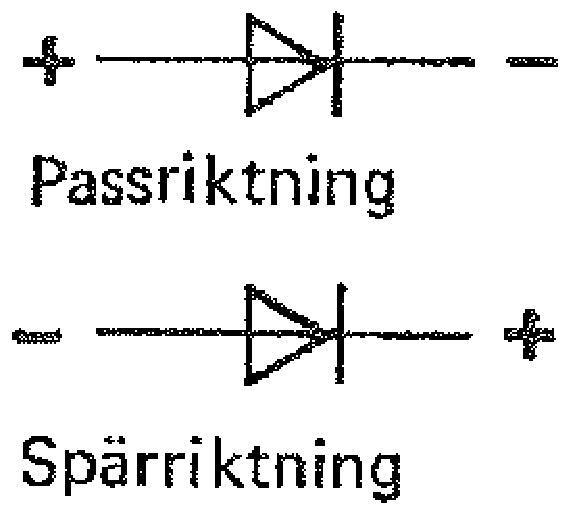
\includegraphics[width=0.5\textwidth]{images/cropped_pdfs/bild_2_3-34.pdf}
\caption{Halvledardioder}
\label{fig:BildII3-34}
\end{wrapfigure}

\emph{Likriktning} (eng. \emph{rectificiation}) av spänningar och strömmar i en
krets görs med ''elektroniska ventiler'' som släpper igenom ström endast i den
så kallade passriktningen och stoppar i spärriktningen så som illustreras i
bild \ref{fig:BildII3-34}.
En sådan strömventil kallas för diod och kan vara av typen vakuumrör eller
halvledare.
I moderna konstruktioner används uteslutande halvledardioder i
likriktarkopplingar.

\begin{figure}
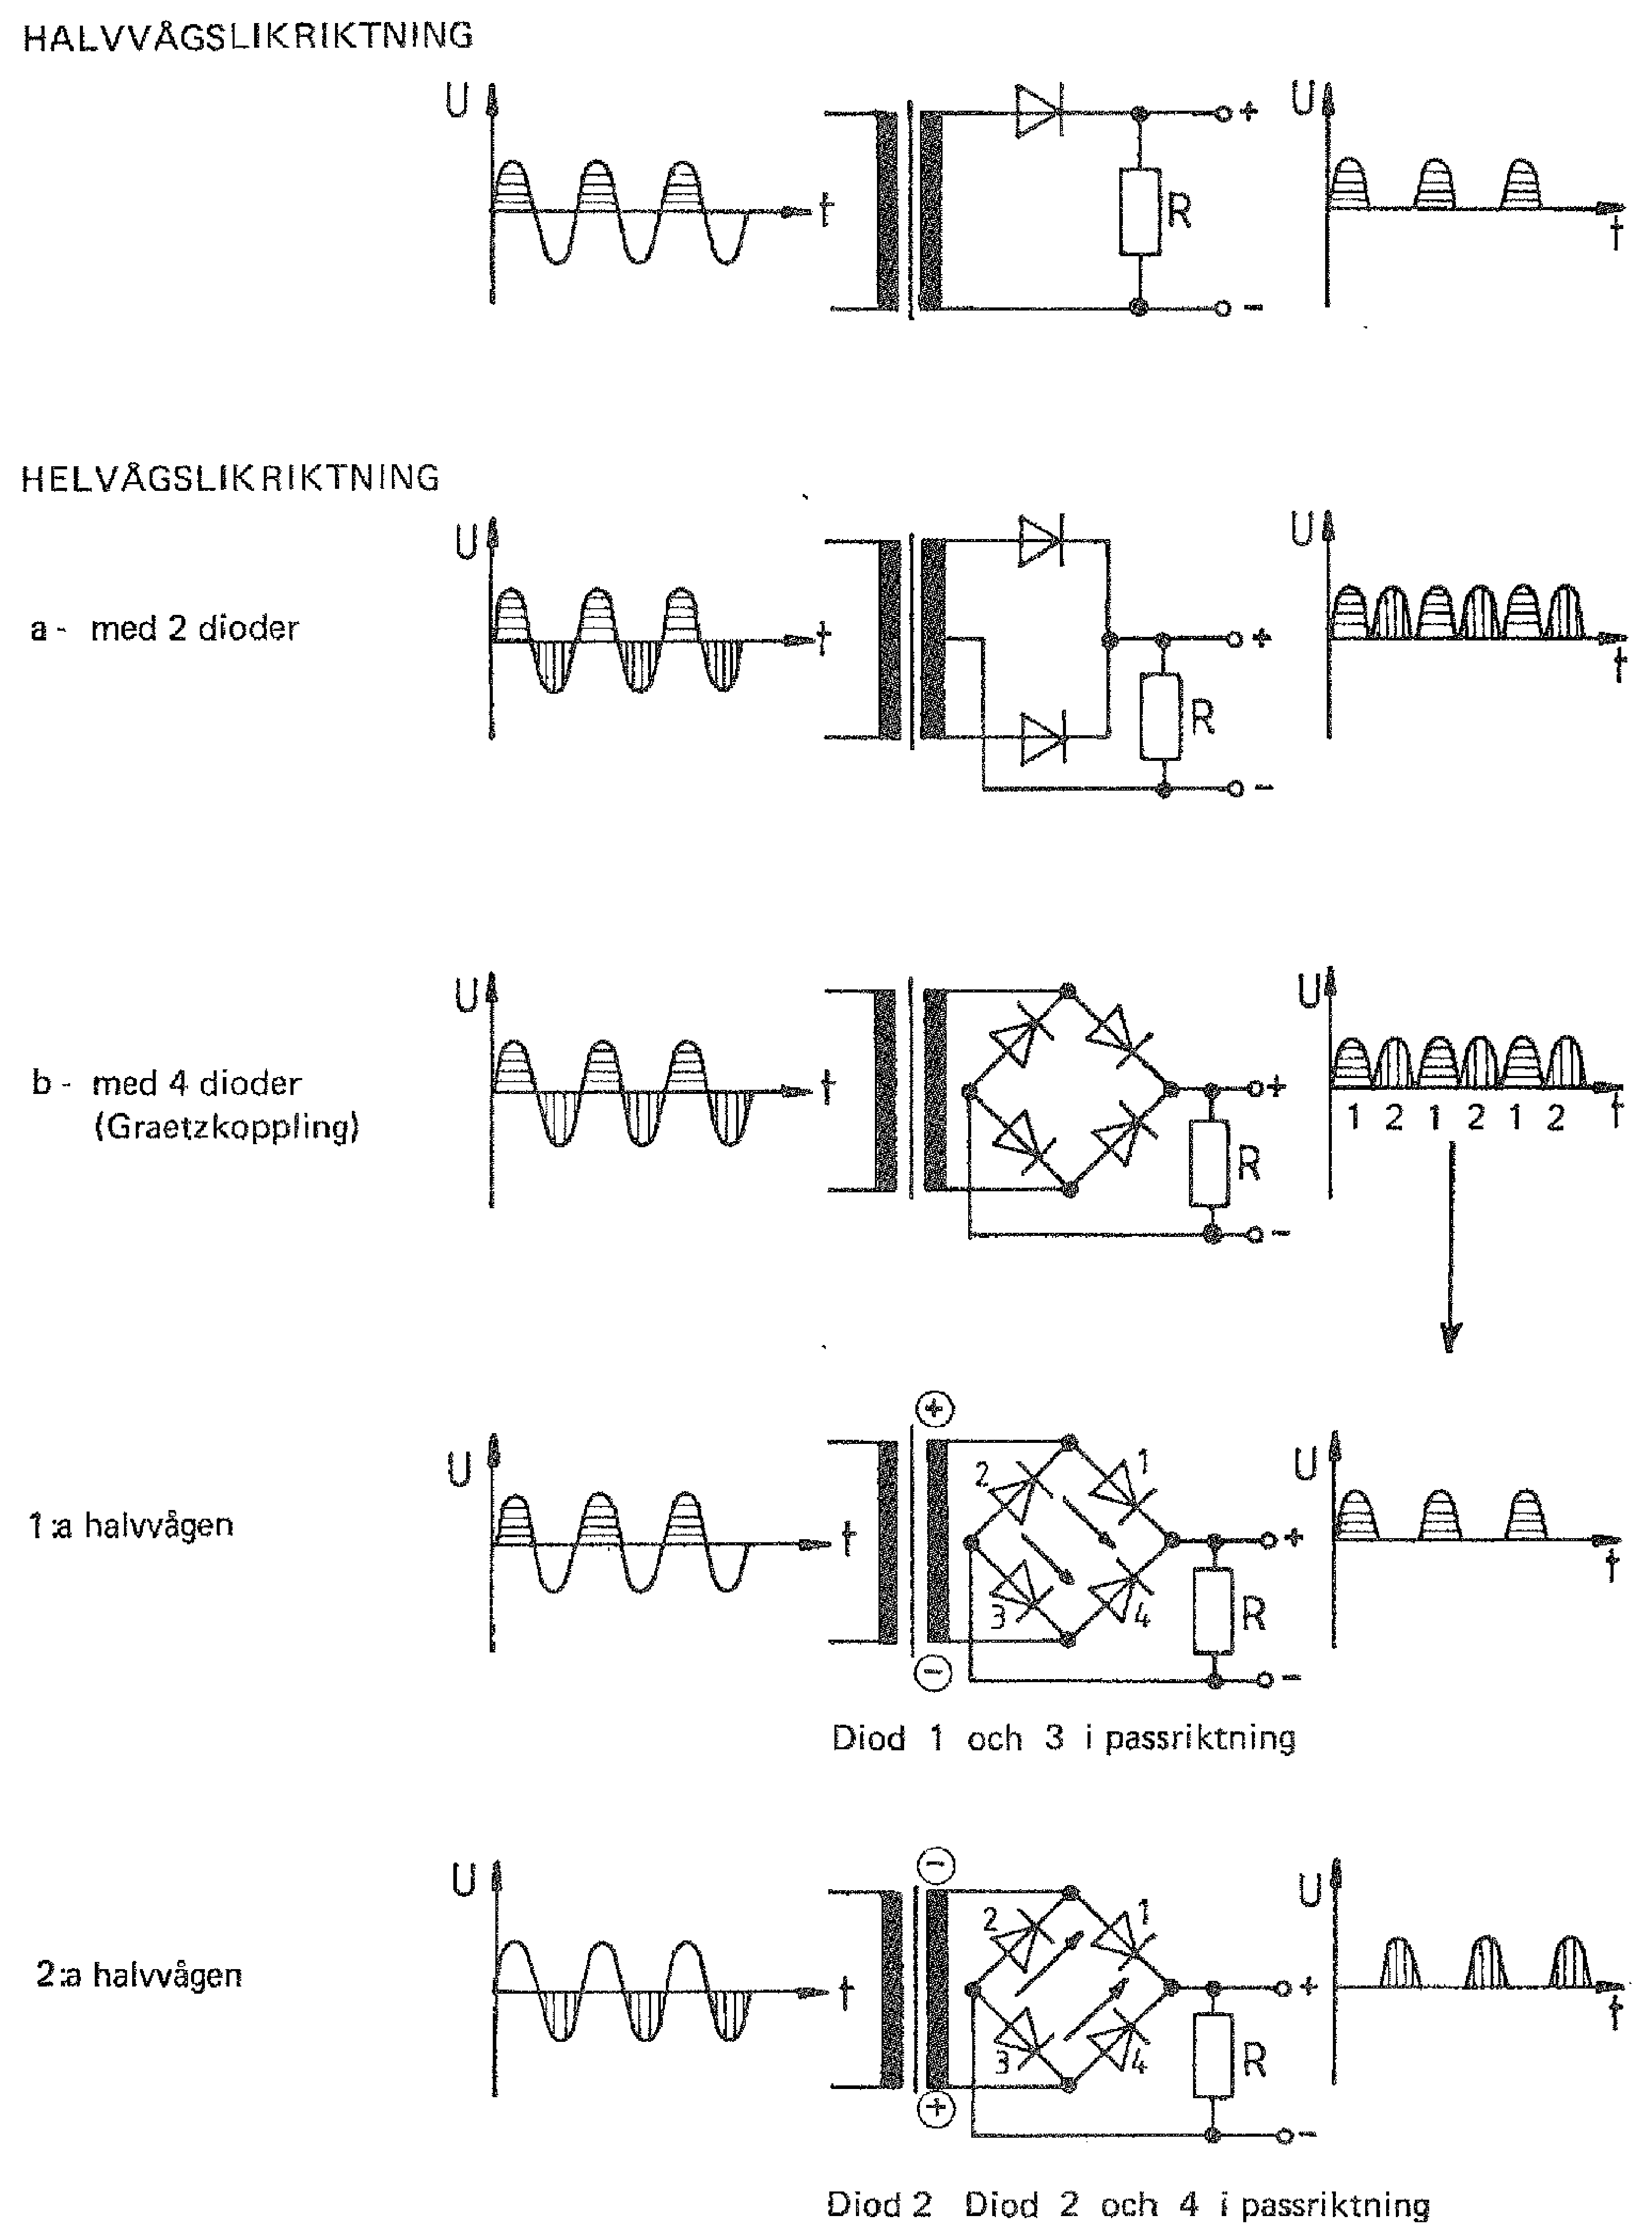
\includegraphics[width=\textwidth]{images/cropped_pdfs/bild_2_3-35.pdf}
\caption{Halv- och helvågslikriktning}
\label{fig:BildII3-35}
\end{figure}

\subsubsection{Halvvågslikriktning}
\index{halvvågslikriktning}
\index{likriktning!halvvågs}

Vid \emph{halvvågslikriktning} (eng. \emph{half wave rectification}) släpps endast
varannan halvvåg av en växelspänning igenom.
I den strömkrets som bildas av transformatorns sekundärlindning, dioden och
lasten, flyter därför ström endast under varannan halvperiod, så som
illustreras i bild \ref{fig:BildII3-35}.

\subsubsection{Helvågslikriktning}
\index{helvågslikriktning}
\index{likriktning!helvågs}
\index{Graetz-brygga}
\index{likriktning!Graetz-brygga}

I följande kopplingar med två respektive fyra dioder släpps varje halvvåg av
transformatorns växelspänning igenom så att alla halvvågor får samma polaritet.
Ström flyter genom lasten i samma riktning under varje halvperiod.
Följande sätt att anordna \emph{helvågslikriktning}
(\emph{full wave rectification}) är vanliga:
\begin{itemize}
\item Med två dioder och mittuttag på transformatorns sekundärlindning.
  Den ena dioden och ena lindningshalvan släpper igenom ström till lasten
  under ena halvperioden.
  Den andra dioden och andra lindningshalvan under den följande halvperioden.
  Detta illustreras i bild \ref{fig:BildII3-35}, delfigur a.

\item Med fyra dioder (s.k. Graetz-brygga) och inget mittuttag på
  transformatorns sekundärlindning släpper dioderna 1 och 3 igenom
  ström under den ena halvperioden.
  Dioderna 2 och 4 släpper igenom ström under den följande halvperioden.
  Detta illustreras i bild \ref{fig:BildII3-35}, delfigur b samt 1:a och 2:a
  halvvågen.
\end{itemize}

\subsection{Glättningskretsar}
\textbf{HAREC a.\ref{HAREC.a.3.3.2}\label{myHAREC.a.3.3.2}}
\index{glättning}
\index{kraftaggregat!glättning}
\index{säkerhetsresistor}
\index{bleeder}

\begin{figure}
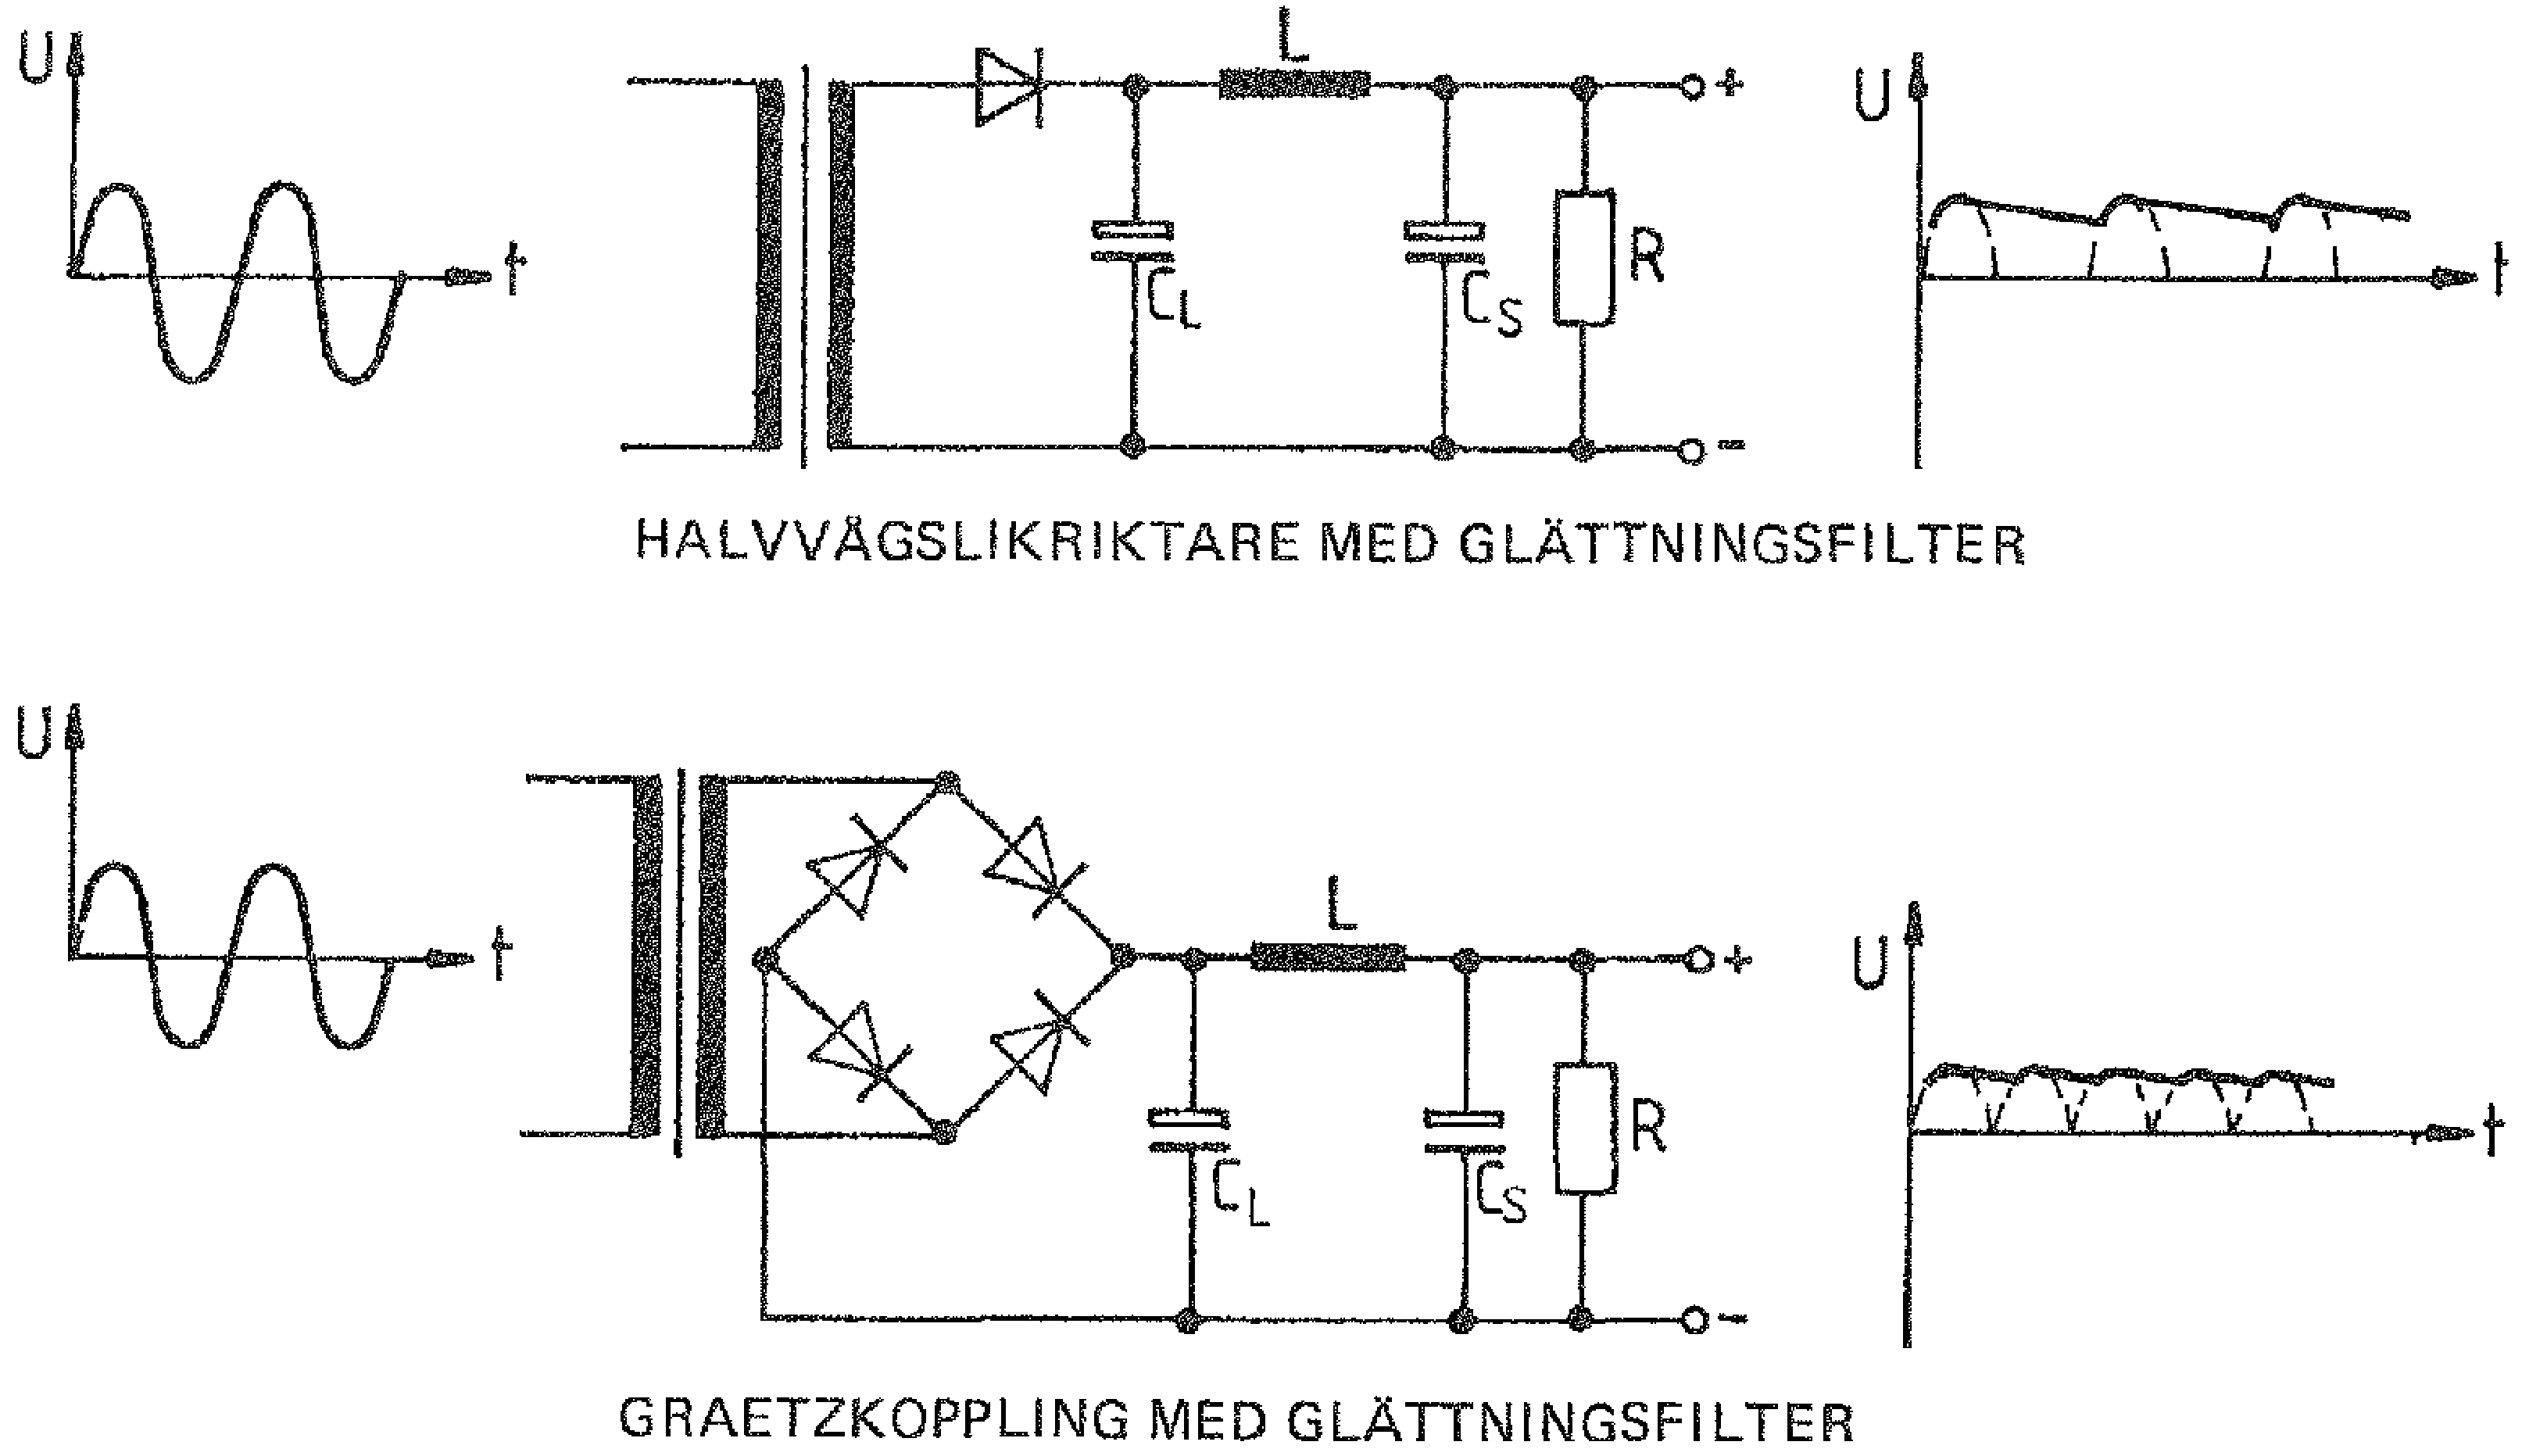
\includegraphics[width=\textwidth]{images/cropped_pdfs/bild_2_3-36.pdf}
\caption{Glättning av likspänning}
\label{fig:BildII3-36}
\end{figure}

Efter likriktningen har växelspänningen omvandlats till en pulserande
likspänning som kan ''glättas''.
Efter likriktarna ansluts då ett filter som utför \emph{glättning}.
Glättningsfiltret kan till exempel bestå av laddningskondensatorn \(C_L\), induktansen \(L\) och glättningskondensatorn \(C_S\) så som bild \ref{fig:BildII3-36}
illustrerar.
Parallellt över denna kondensator ligger för elsäkerhetens skull en
urladdningsresistor \(R\) med hög resistans alltid inkopplad.

\emph{Säkerhetsresistorn} (eng. \emph{bleeder}) ska ladda ur kondensatorerna,
när kraftaggregatet är obelastat och inte anslutet till strömförsörjningen på primärsidan.
Säkerhetsresistorn ska vara av trådlindad typ och kunna tåla fyra gånger sin
egen effektförbrukning.

I obelastat tillstånd är spänningen över laddningskondensatorn \(\sqrt{2}\)
gånger större än effektivvärdet på transformatorns sekundärspänning.
När en transformator i tomgång har ett effektivvärde av 230~V över
sekundärlindningen blir spänningen över säkerhetsmotståndet
\(230\cdot\sqrt{2} \approx 325\)~V.

\subsubsection{Spänningshöjande likriktarkopplingar}
\index{kraftaggregat!spänningshöjning}
\index{kraftaggregat!spänningsdubbling}

Vid likriktning av växelspänningar enligt någon av ovanstående metoder behövs
en sekundärspänning från transformatorn av minst samma storlek som den önskade
likspänningen.
Önskas en högre likspänning, till exempel den dubbla, men med samma sekundärspänning
på transformatorn, så kan en speciell likriktarkoppling användas.

\begin{figure}
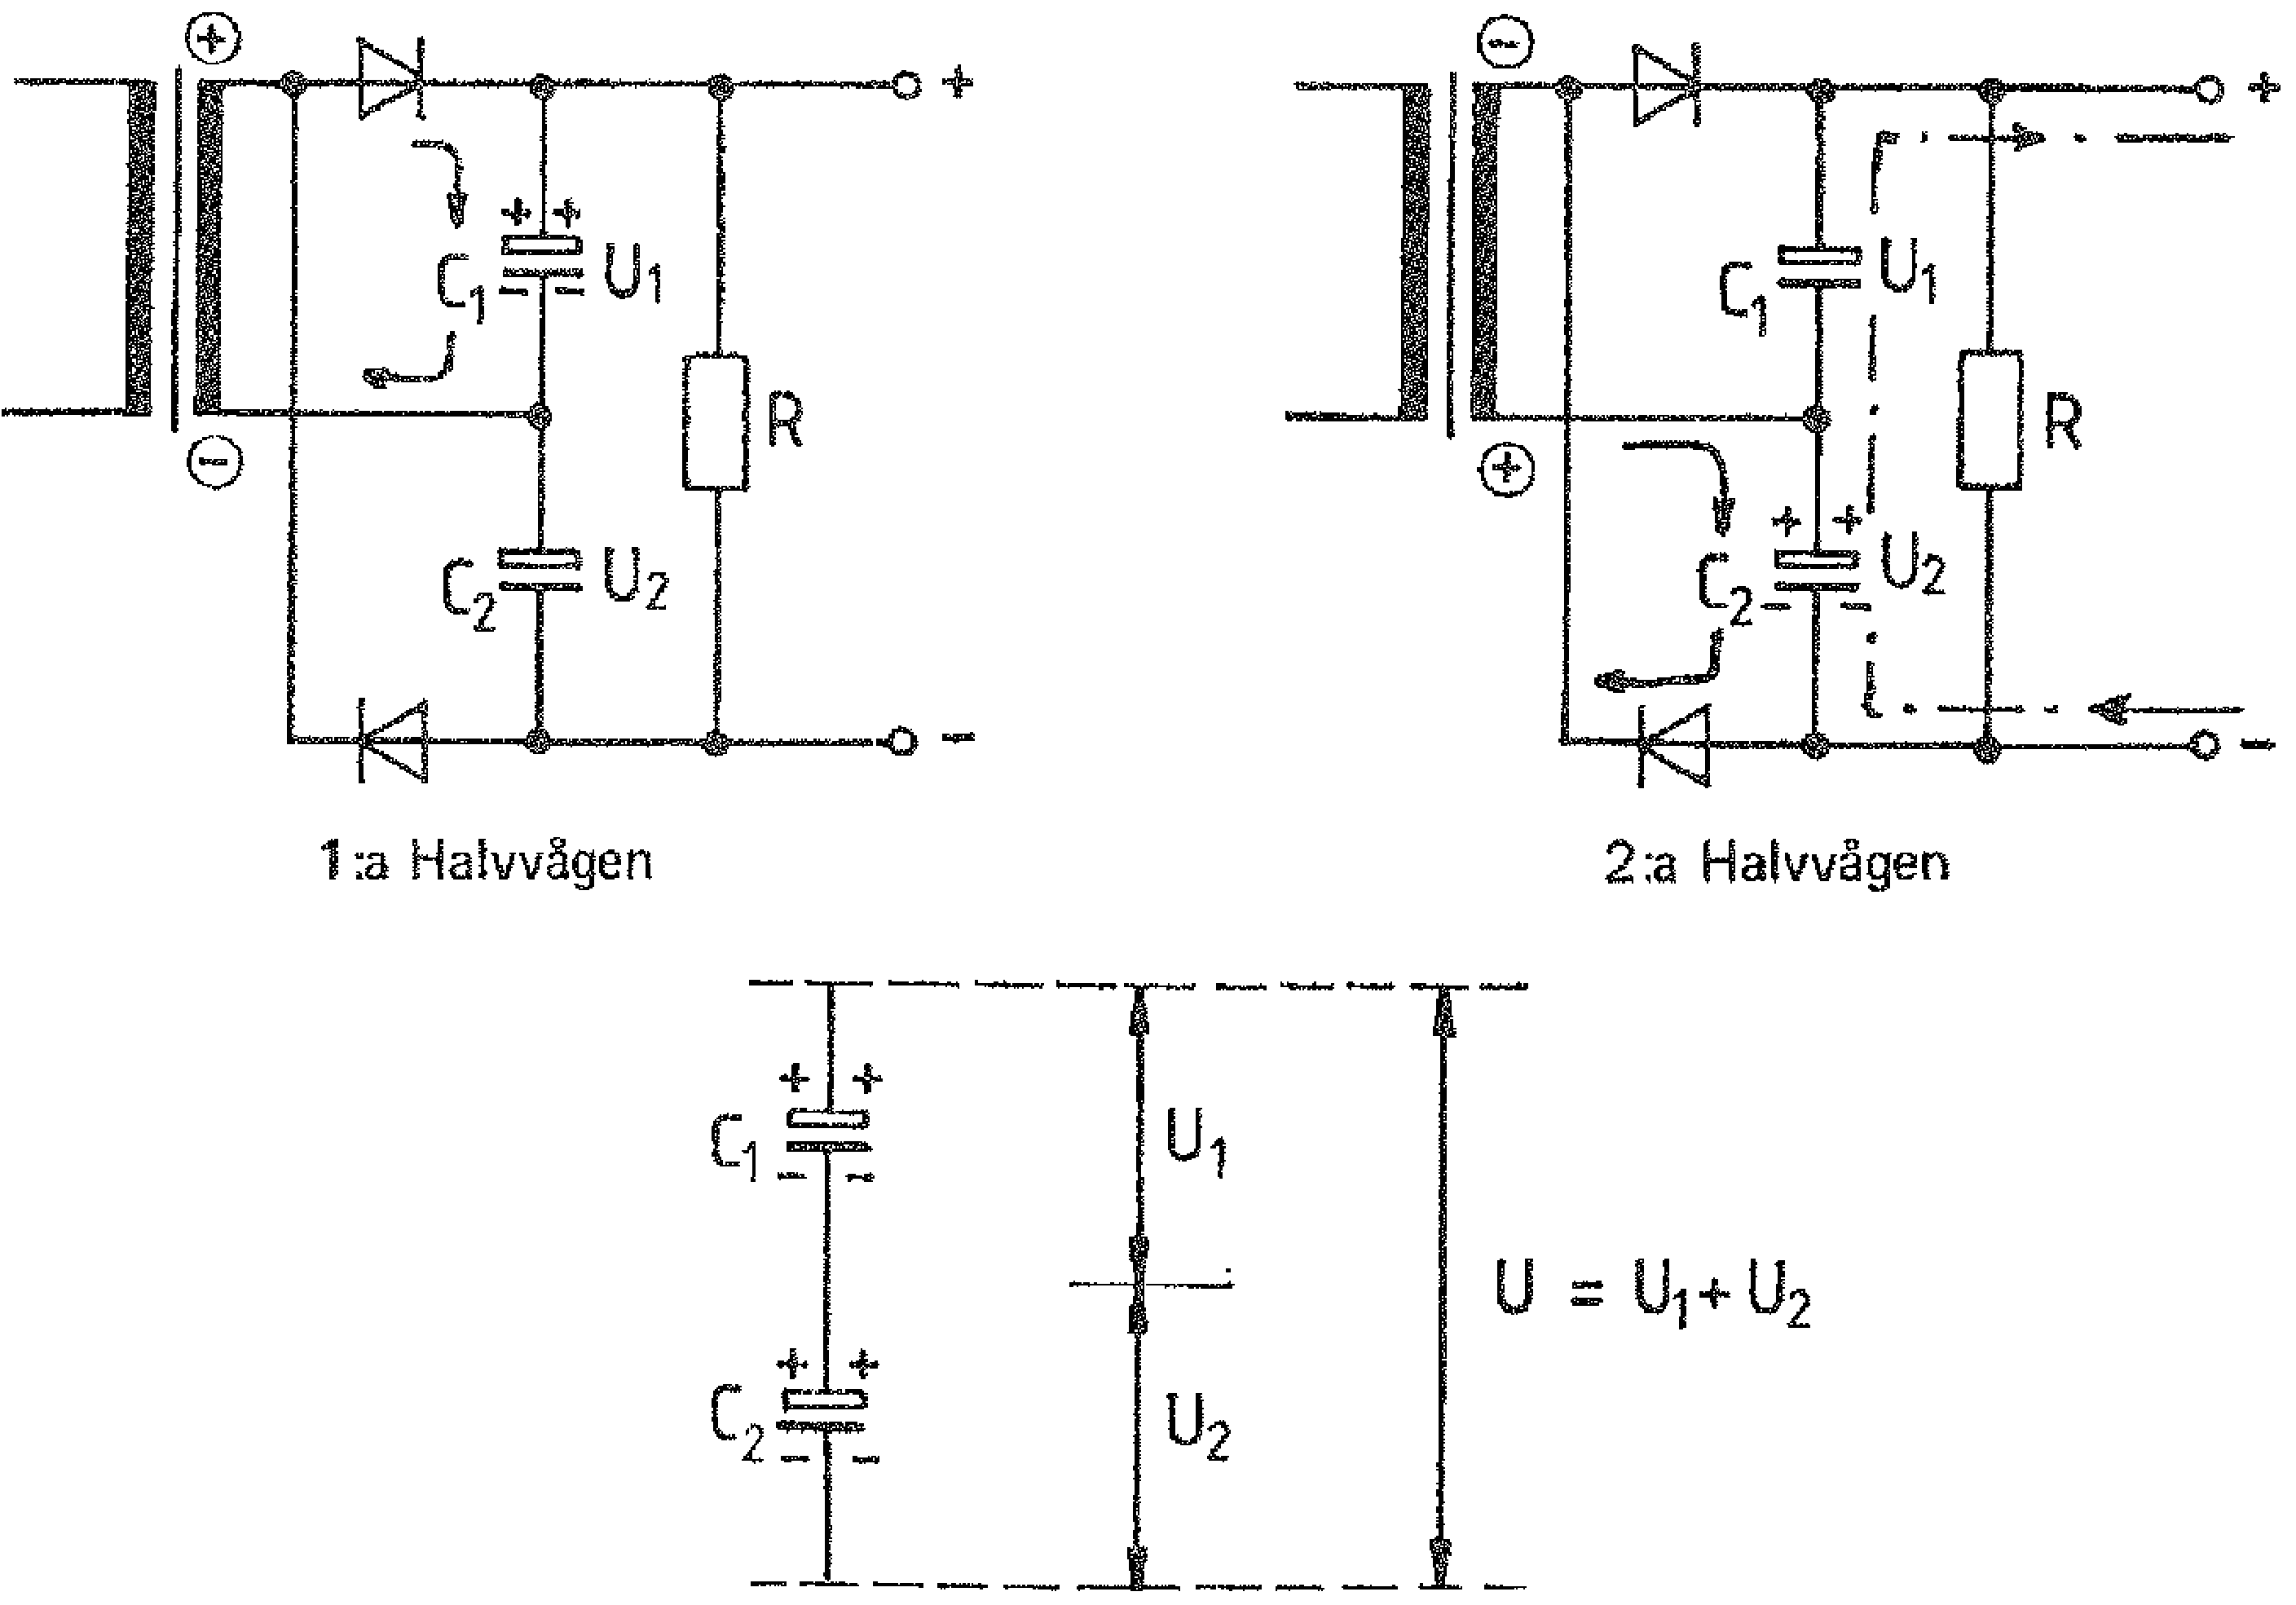
\includegraphics[width=\textwidth]{images/cropped_pdfs/bild_2_3-37.pdf}
\caption{Likriktarkoppling med spänningsdubbling}
\label{fig:BildII3-37}
\end{figure}

Bild \ref{fig:BildII3-37} visar en spänningsdubblande koppling.
Under 1:a halvvågen laddas kondensator \(C_1\) upp.
Under 2:a halvvågen laddas kondensator \(C_2\) upp.
Kondensatorerna är kopplade i serie och den ena kondensatorn hinner inte bli
urladdad under tiden som den andra kondensatorn blir uppladdad.
Följden blir att belastningen ser kondensatorernas spänningar som seriekopplade
och därmed har en fördubbling av spänningen erhållits.
Det finns även kopplingar för flerdubbling av spänningar, vilka bland annat
brukade användas för att alstra accelerationsspänningen för TV-bildrör.

\subsection{Spänningsstabilisering}
\textbf{HAREC a.\ref{HAREC.a.3.3.3}\label{myHAREC.a.3.3.3}}
\index{spänningsstabilisering}
\index{kraftaggregat!spänningsstabilisering}

\begin{wrapfigure}{R}{0.5\textwidth}
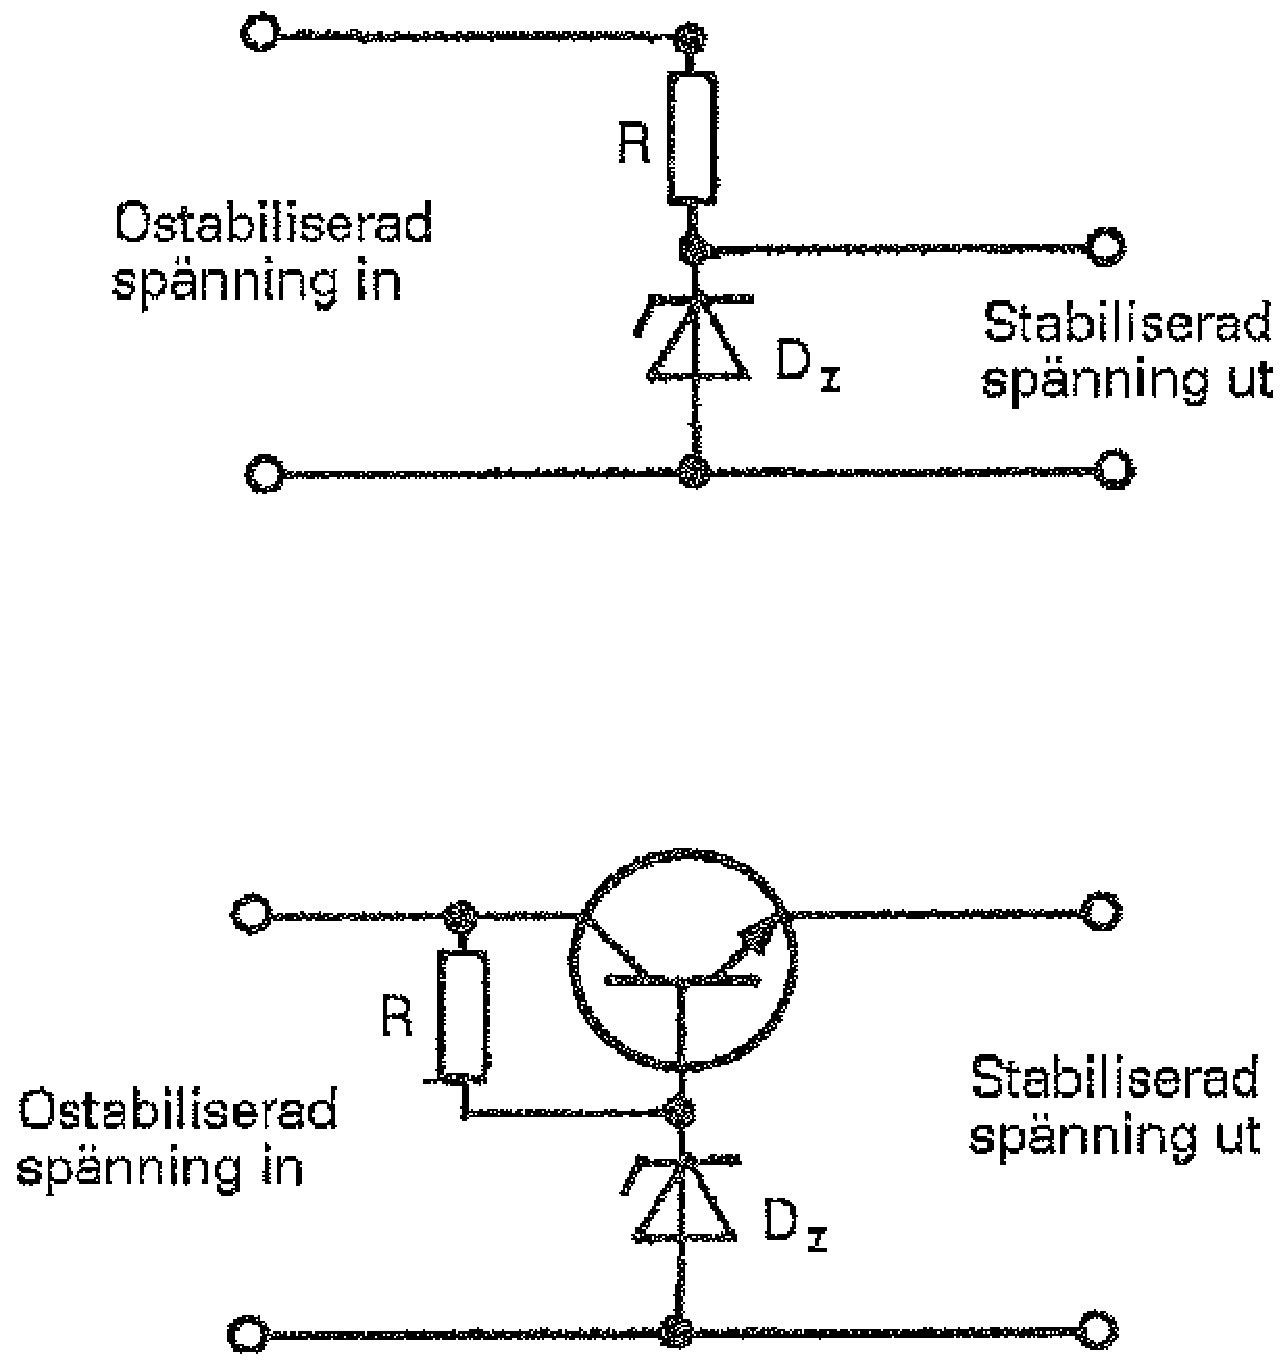
\includegraphics[width=0.5\textwidth]{images/cropped_pdfs/bild_2_3-38.pdf}
\caption{Spänningsstabilisering}
\label{fig:BildII3-38}
\end{wrapfigure}

Utspänningen från ett kraftaggregat tillåts i många fall endast att variera
mellan vissa värden, även om inspänningen och strömuttaget varierar mycket.
Ett vanligt sätt att hålla konstant spänning är att efter glättningsfiltret anordna en stabiliseringskrets, som visas i bild \ref{fig:BildII3-38}.

Glimlampan och zenerdioden har egenskapen att spänningsfallet över dem är i det
närmaste konstant inom ett visst strömområde.
Glimlampor arbetar på högre spänningar och används i utrustningar med
elektronrör.
Zenerdioder arbetar på de lägre spänningar som används i dagens elektronik.

Stabiliseringen tillgår så att till exempel zenerdioden får ingå som aktiv del
i en spänningsdelare, som består av en resistor i serie med belastningen och
zenerdioden parallellt med den.
Zenerdioden tar upp variationerna i belastningsströmmen, varvid spänningen över
spänningsdelarens uttag blir stabiliserad.
Vid större strömuttag kan zenerdioden inte ensam ta upp hela den effekt som den
reglerar bort.
I stället tas effekten upp av en eller flera transistorer som i sin tur
regleras av zenerdioden.

I vissa fall behövs i stället en reglerad utström från kraftaggregatet.
Även för detta ändamål används kopplingar med zenerdioder och transistorer.

Färdiga stabiliseringskretsar i form av integrerade kretsar är numera vanligare än sådana som är uppbyggda av diskreta komponenter. Exempel är linjära spänningsregulatorer som 7805 för 5 V och 7912 för -12 V.

\subsection{Switchaggregat}
\textbf{HAREC a.\ref{HAREC.a.3.3.4}\label{myHAREC.a.3.3.4}}
\index{switchaggregat}
\index{kraftaggregat!switchaggregat}

Senare utvecklingsformer är så kallade switchade aggregat.
I sådana regleras spänningen eller strömmen genom sönderhackning (switching).
Genom att förändra förhållandet mellan till- och frånslagstiderna kan man skapa
det önskade medelvärdet.
Metoden ger hög verkningsgrad.
Switchfrekvensen är i storleksordningen 20~kHz eller högre.
Sådana kraftaggregat kan emellertid ge upphov till radiofrekventa störningar, varför effektiv avstörning
behövs.

Kraftaggregat som omvandlar från nätspänning till likspänning använder
den primärswitchade principen.
I ett primärswitchat aggregat likriktas nätspänningen och switchas på
primärssidan av transformatorn.
Eftersom frekvensen är relativt hög och inte riskerar mätta transformatorns kärna på samma sätt som vid nätfrekvensen (50~Hz), behöver kärnan inte vara så stor.
På sekundärsidan likriktas sedan spänningen och glättning kan ske med relativt
små kondensatorer tack vare den höga frekvensen.
Genom att återkoppla spänningen till primärsidan kan utspänningen regleras i
primärswitchningen istället för att behöva stabiliseras på
sekundärsidan. Därigenom kan förluster i stabiliseringskretsen undvikas.
Ett primärswitchat aggregat måste ha nätfilter för att klara EMC-kraven.

En annan kategori av switchade aggregat används för likspänningsomvandling, så kallad DCDC-omvandling.
Exempel på sådana är kallade drop-omvandlare, som kan används för att sänka spänningen.
Andra omvandlare kan höja spänningen eller byta polaritet på den.
Dessa omvandlare arbetar inte sällan med frekvenser på 200~kHz till 2~MHz.
Likspänningsomvandlare har inte alltid galvanisk isolation mellan in- och utgång.

Numera finns även switchade ersättare med lägre effektförlust än i de äldre linjära regulatorerna i 78- och 79-serien.
Problemet med dessa är att de kan generera störningar som behöver tas hänsyn till.

Switchade kraftaggregat och spänningsstabilisatorer är nu en vanliga eftersom effektförlusterna kan hållas mycket lägre än i gamla linjära aggregat.
Switchningen innebär dock att störningar kan läcka ut både på ingång och utgång såväl som genom direktutstrålning från själva aggregatet.
På en del switchade nätaggregat kan switchfrekvensen justeras manuellt med en ratt. På så sätt kan man flytta störningarna till en frekvens där deras inverkan minskar.
Störningar kan uppträda både i differentiell och gemensam mode, vilket man måste ta hänsyn till vid avstörning.